%Version 3.1 December 2024
%
%%%%%%%%%%%%%%%%%%%%%%%%%%%%%%%%%%%%%%%%%%%%%%%%%%%%%%%%%%%%%%%%%%%%%%
%% Supplementary Information in the Springer Nature LaTeX template %%
%% layout (class file sn-jnl.cls, unmodified). Submitted as one    %%
%% PDF: figures, then tables, then text.                           %%
%%%%%%%%%%%%%%%%%%%%%%%%%%%%%%%%%%%%%%%%%%%%%%%%%%%%%%%%%%%%%%%%%%%%%%

\documentclass[pdflatex,sn-nature]{sn-jnl}% Style for submissions to Nature Portfolio journals

%%%% Standard Packages
\usepackage{graphicx}%
\usepackage{multirow}%
\usepackage{amsmath,amssymb,amsfonts}%
\usepackage{amsthm}%
\usepackage{mathrsfs}%
\usepackage[title]{appendix}%
\usepackage{xcolor}%
\usepackage{textcomp}%
\usepackage{manyfoot}%
\usepackage{booktabs}%
\usepackage{algorithm}%
\usepackage{algorithmicx}%
\usepackage{algpseudocode}%
\usepackage{listings}%
\usepackage{bm}% additional package required by this document (bold math symbols)
%%%%

\raggedbottom
\unnumbered% unnumbered level heads, as in Nature Portfolio journals
\setcitestyle{numbers,square,comma,sort&compress}
%% Figures are found either beside this file or in figures/ (Overleaf project).

% SI citations restart from 1 and have their own complete embedded list.
\renewcommand{\refname}{Supplementary References}

\begin{document}

\title{Supplementary Information: Resonant enhancement and source priors shape subwavelength acoustic reconstruction}

\author[1,3]{\fnm{Nurtugan} \sur{Rysmambetov}}\nomail
\author[2,3]{\fnm{Zhanat} \sur{Kappassov}}\nomail
\author[1,3]{\fnm{Bakhtiyar} \sur{Orazbayev}}\nomail
\affil[1]{\orgdiv{Department of Physics}, \orgname{Nazarbayev University}, \orgaddress{\city{Astana}, \country{Kazakhstan}}}
\affil[2]{\orgdiv{School of Computing and Artificial Intelligence}, \orgname{Nazarbayev University}, \orgaddress{\city{Astana}, \country{Kazakhstan}}}
\affil[3]{\orgdiv{Robotics Center}, \orgname{Institute of Smart Systems and Artificial Intelligence, Nazarbayev University}, \orgaddress{\city{Astana}, \country{Kazakhstan}}}

\maketitle

% Keep short columns from stretching the spaces around headings and paragraphs.
\raggedbottom

\setcounter{figure}{0}
\setcounter{equation}{0}
\renewcommand{\thefigure}{\arabic{figure}}
\renewcommand{\figurename}{Supplementary Figure}
\renewcommand{\tablename}{Supplementary Table}
\renewcommand{\thetable}{\arabic{table}}
\renewcommand{\theequation}{\arabic{equation}}

\clearpage

\begin{figure}[p]
\centering
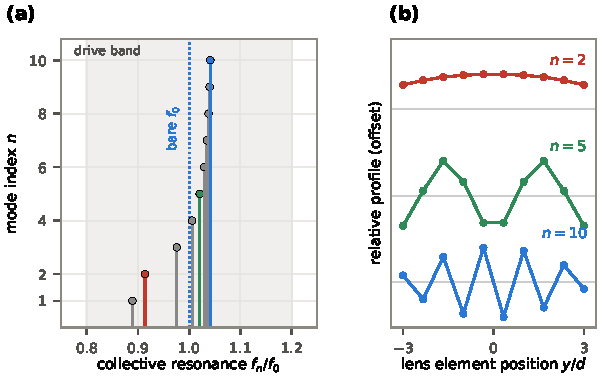
\includegraphics[width=.68\textwidth]{figures/supplement/figS2_lensmodes.pdf}%
\caption{\label{fig:modes}%
Approximate collective lens resonance frequencies $f_n$, normalized by reference lens resonance $f_0$, with the coupling evaluated at $f_0$ (Note~3). (a)~Frequencies of the ten modes, with the drive band shaded and
uncoupled frequency dotted. (b)~Real parts of three selected lens-mode profiles,
$n=2,5,10$, indexed by increasing resonance frequency, scaled to their own maxima and vertically offset.
Here $y$ is position along the lens, $d$ is source pitch and $y/d$ gives that position in source-pitch units.}

\end{figure}
\clearpage

\begin{figure}[p]
\centering
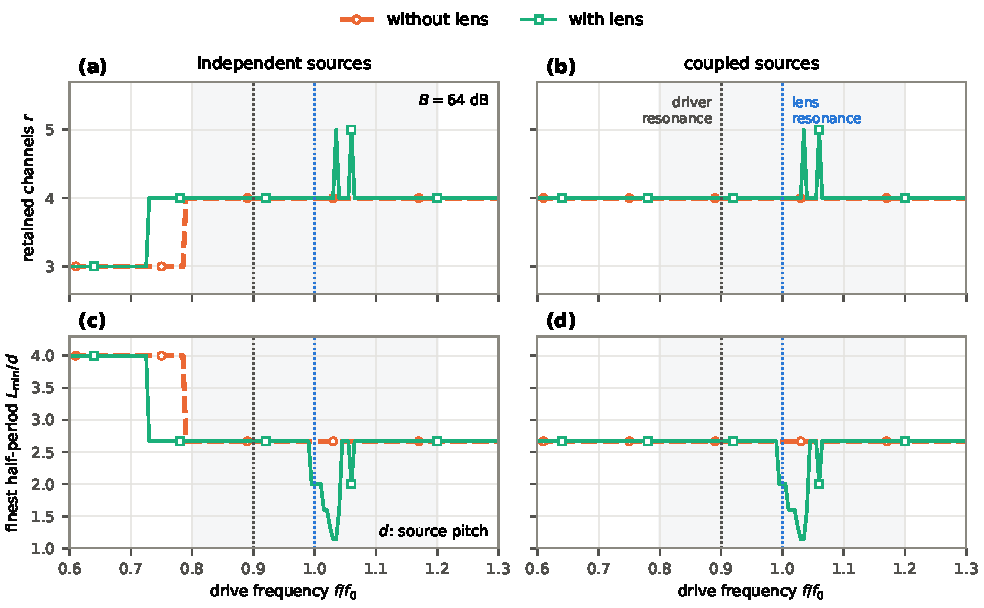
\includegraphics[width=.90\textwidth]{figures/supplement/figS3_freqsweep.pdf}%
\caption{\label{fig:fsweep}%
Single-frequency retained channels and cosine-pattern capture at relative measurement budget $B=20\log_{10}(\sigma_1/\sigma_n)=64$~dB, where $\sigma_1$ is the strongest singular gain and $\sigma_n$ the model noise standard deviation. The drive frequency $f$ sweeps across $0.6$--$1.3\,f_0$, with reference lens resonance $f_0$ (drive band shaded).
(a,b)~Retained channel count $r$; (c,d)~finest passing cosine half-period $L_{\min}$, shown in source-pitch units $d$, with $C_m\geq0.5$, where $C_m$ is the fraction of squared source norm retained for unit cosine probe $m$.
Left/right columns use independent/coupled sources. Independent sources omit source--source scattering and lens feedback; coupled sources retain both (Note~1).
Dotted lines mark driver and lens resonances.
Markers distinguish coincident curves.}

\end{figure}
\clearpage

\begin{figure}[p]
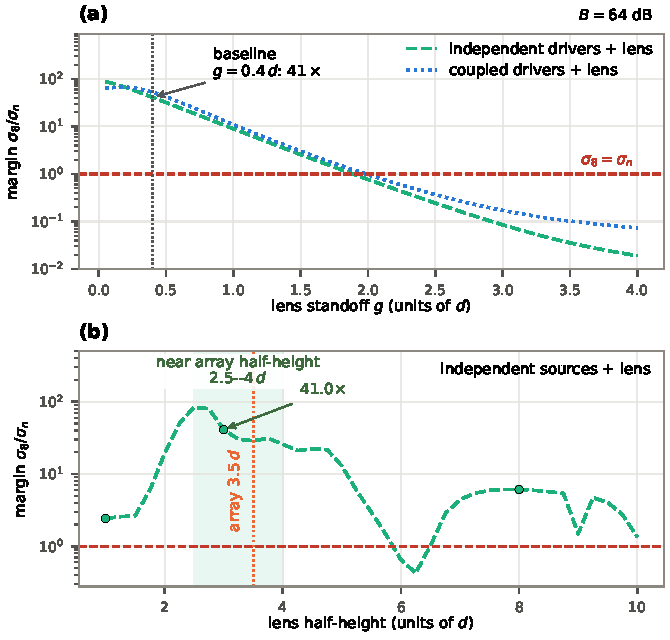
\includegraphics[width=.65\textwidth]{figures/supplement/figS4_install.pdf}%
\caption{\label{fig:install}%
Model margin $\sigma_8/\sigma_n$, the weakest singular gain divided by the model noise standard deviation, at relative budget $B=64$~dB; the dashed horizontal level is $1$.
(a)~Source--lens standoff; the dotted line marks the baseline value. (b)~Lens half-height at fixed element count; shading marks $2.5$--$4\,d$, and the dotted line marks the source-array half-height $3.5\,d$. Independent sources with the lens,
except the coupled-source comparison in (a). Here $d$ is source pitch.}

\end{figure}
\clearpage

\begin{figure}[p]
\centering
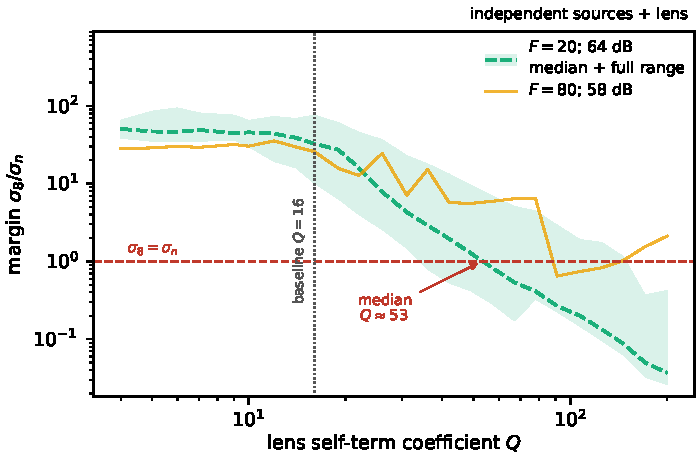
\includegraphics[width=0.62\textwidth]{figures/supplement/fig_q_sweep.pdf}%
\caption{\label{figS:qsweep}%
Weakest-channel margin $\sigma_8/\sigma_n$ versus the resonant self-term coefficient $Q$ on fixed tone grids (independent sources); the relation between $Q$ and loaded quality factor is given in Note~1.
Here $F$ is the number of drive tones. For $F=20$, shading spans ten frequency shifts and the median margin crosses one near $Q\approx53$.
The $F=20$ curves use a $64$ dB relative budget; the $F=80$ curve uses $58$ dB. At the same strongest-gain normalization, the latter increases the assumed per-sample noise-to-gain ratio by a factor of $2$. The comparison changes both the tone grid and relative noise level.}

\end{figure}
\clearpage

\begin{figure}[p]
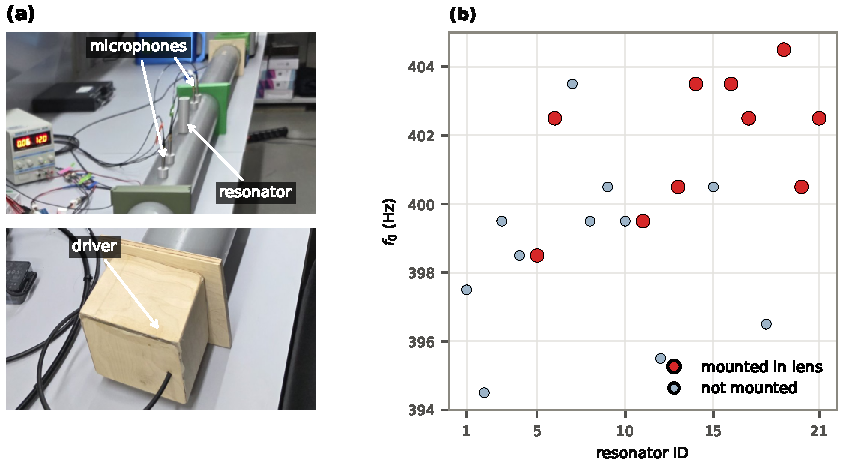
\includegraphics[width=0.80\textwidth]{figures/supplement/figS5_qscatter.pdf}%
\caption{\label{figS:qscatter}%
Resonator characterization. (a)~Four-microphone impedance tube (two-source method,
ASTM E2611): microphone/resonator region above and driver below, from one photograph.
(b)~Resonance frequencies of 21 elements; the ten mounted in the lens are marked separately.}

\end{figure}
\clearpage

\begin{figure}[p]
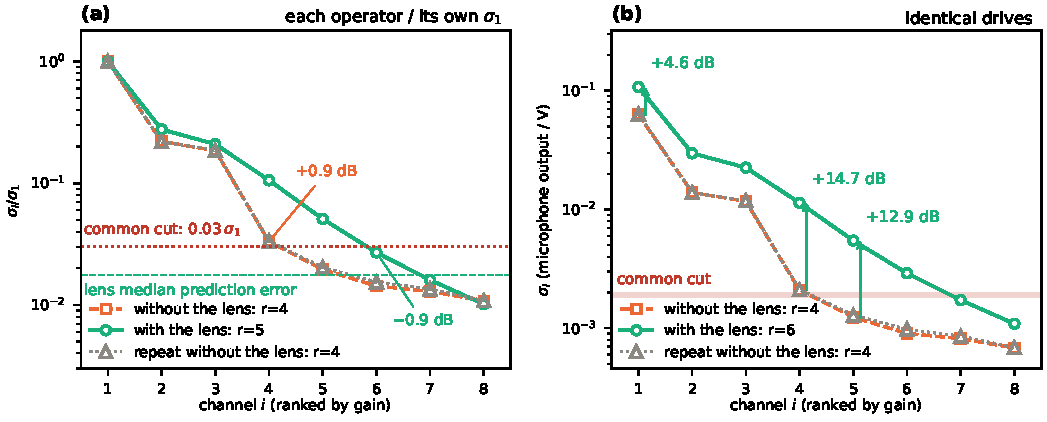
\includegraphics[width=\textwidth]{figures/supplement/fig_measured_budget_rewrite.pdf}%
\caption{\label{figS:budget}%
Measured singular spectra of the unweighted per-volt operator $H_V$. (a)~Normalized by each operator's strongest singular gain $\sigma_1$;
empirical spectral cutoff $0.03\,\sigma_1$ (dotted) sets the counts.
Dashed: lens-session median recording prediction error.
(b)~Unnormalized spectra at identical drives. Shading spans reference levels obtained by multiplying each operator's strongest singular gain by its session's median relative prediction error (Note~10); the largest level sets the common cutoff for the reported counts.
Arrows compare singular gains at the same ordered index; the corresponding source patterns can differ between operators.}

\end{figure}
\clearpage

\begin{figure}[p]
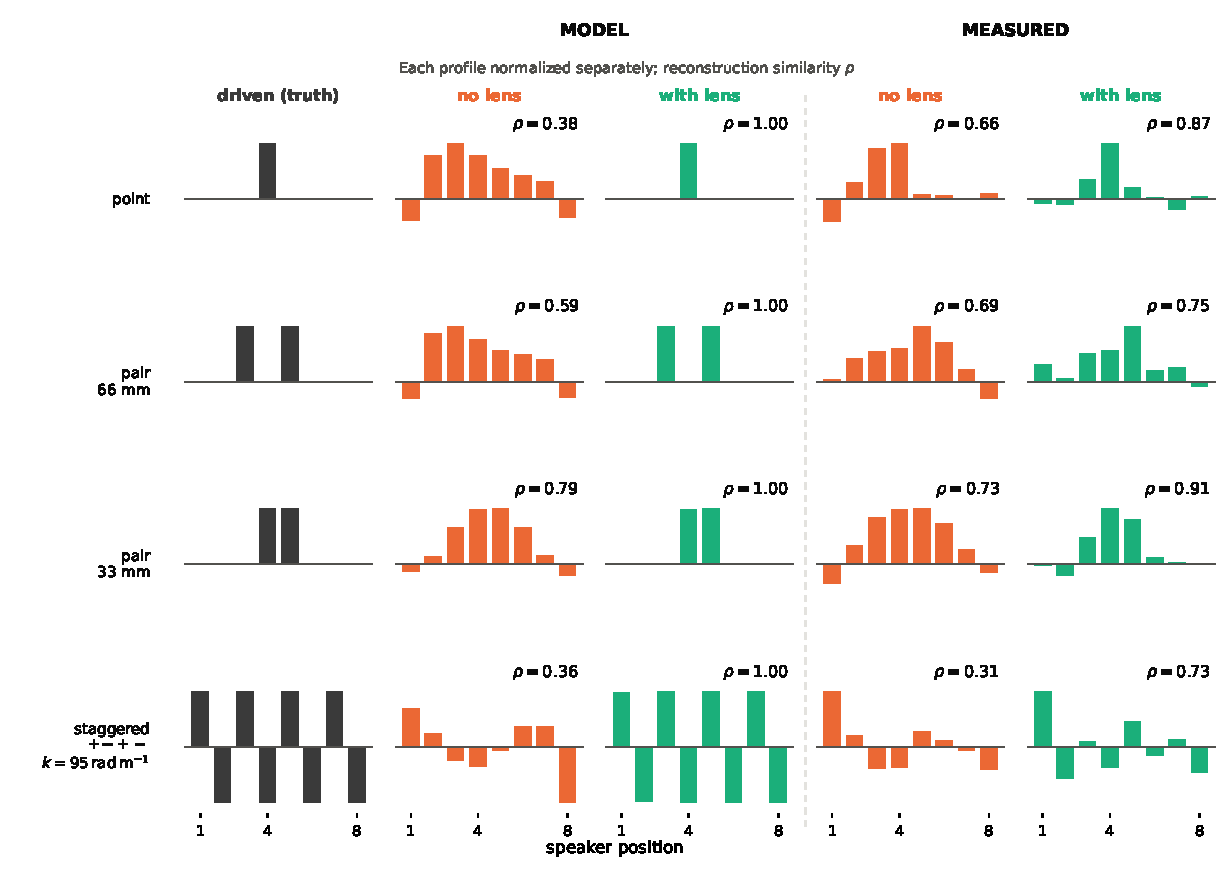
\includegraphics[width=\textwidth]{figures/supplement/figS6_exprecon.pdf}%
\caption{\label{figS:exprecon}%
Driven profiles and reconstructed profiles without/with the lens. Displayed curves are real parts after the phase and peak normalizations specified in Note~11. Similarity is
$\rho=|\hat{\bm a}^{\dagger}\bm a|/(\|\hat{\bm a}\|\|\bm a\|)$, evaluated on the full complex profiles before display normalization.
Model columns use the coupled-source model, peak-one drives, one noise realization and the $64$~dB reference budget with $\sigma_n=10^{-3}$. The supplementary noise-level cutoff retains five/eight channels without/with the lens; main-text Fig.~2c instead uses floor ranks three/eight and unit-norm drives. Distance and wavenumber labels describe the bench; the model applies the same eight-component patterns on its coarser grid.
Measured columns use eight loudspeakers, six microphones and $41$ tones over $350$--$450$~Hz, retaining four/five channels without/with the lens. Printed similarities average five individual acquisitions; displayed profiles follow the separate repeat-alignment procedure in Note~11.
Main-text Fig.~4 uses a common true-peak display scale and scores unrefitted full complex profiles.}

\end{figure}
\clearpage

\begin{figure}[p]
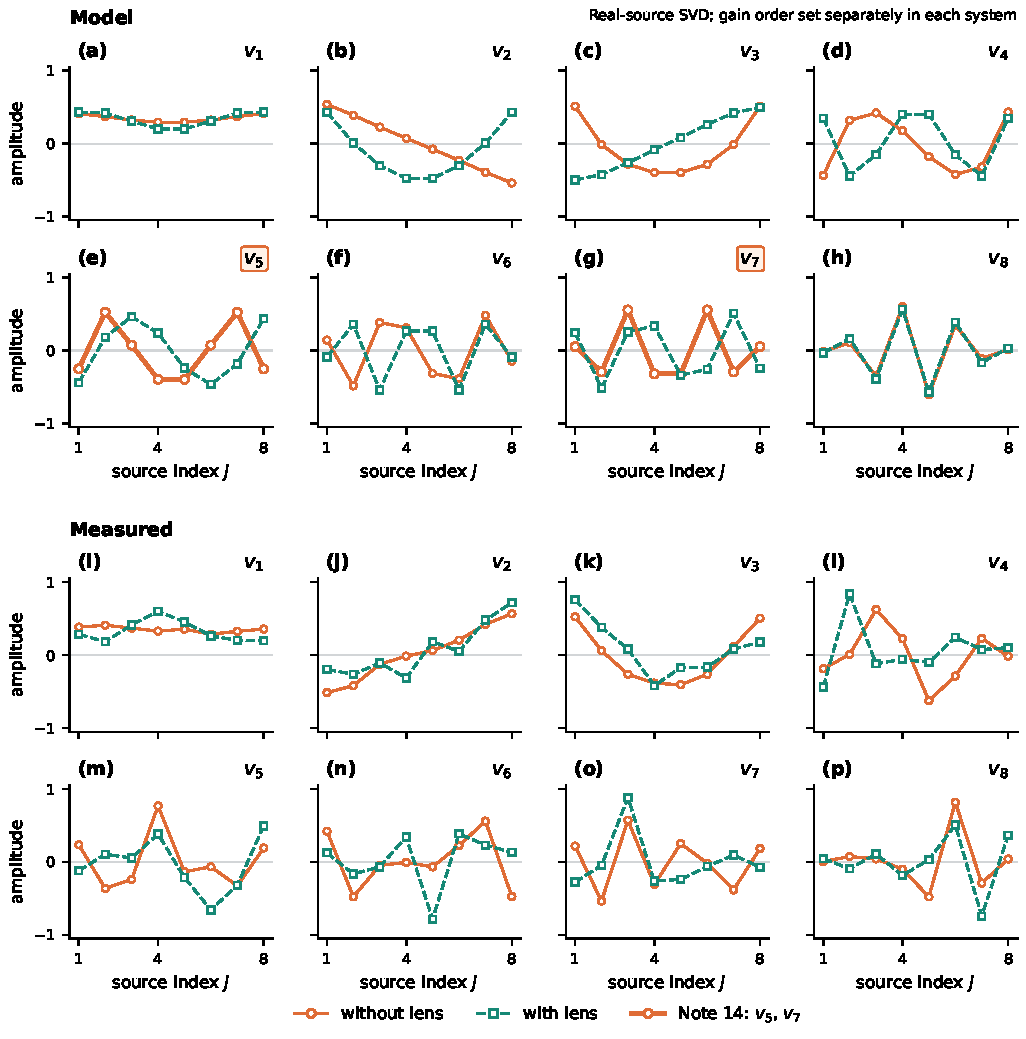
\includegraphics[width=\textwidth]{figures/supplement/fig_singular_patterns.pdf}%
\caption{\label{figS:singularpatterns}%
Unit-norm real-source singular-value decomposition (SVD) patterns $v_1$--$v_8$ at the eight source positions:
(a--h)~model; (i--p)~measured operators. Each basis uses
$[\operatorname{Re}T;\operatorname{Im}T]$, where $T$ maps source drives to microphone recordings, and follows descending gain.
Signs are aligned for display; equal indices need not identify the same spatial pattern.
Thicker orange curves and outlined labels mark the fixed lens-free model patterns
$v_5$ and $v_7$ used in Note~14. Main-text Fig.~5 instead uses the model with-lens patterns $v_3,v_5$ and measured no-lens patterns $v_5,v_7$, with the stated source restrictions.}

\end{figure}
\clearpage


\begin{table}[p]
\centering
\caption{\label{tab:rank_sensitivity}Rank and weighting sensitivity of the recorded-profile score. Entries are the five-record RMS relative profile error $E_{\rm prof}$ of main-text Fig.~4c, recomputed from the frozen complex TSVD returns at hard ranks four to six with the mean calibration operator. The first-weighting column uses the weight array of the displayed profiles; the range is the minimum and maximum over the nine individual-baseline weight arrays, and the last column counts the weightings that meet $E_{\rm prof}\le1/\sqrt2$. Rank five (bold) is the rank used in the main text. The nine weightings reuse the same five recordings and are not independent repeats; the ranges are not confidence intervals.}
\setlength{\tabcolsep}{5pt}
\begin{tabular}{llcccc}
\toprule
Pattern & Arm & Rank & First weighting & Range over weightings & Passing\\
\midrule
$\lambda/6.5$ sine & No lens & 4 & $0.57$ & $[0.34, 0.63]$ & $9/9$ \\
$\lambda/6.5$ sine & No lens & \textbf{5} & $0.73$ & $[0.49, 0.79]$ & $6/9$ \\
$\lambda/6.5$ sine & No lens & 6 & $0.82$ & $[0.72, 1.20]$ & $0/9$ \\
\addlinespace[2pt]
$\lambda/6.5$ sine & With lens & 4 & $0.63$ & $[0.57, 0.63]$ & $9/9$ \\
$\lambda/6.5$ sine & With lens & \textbf{5} & $0.49$ & $[0.44, 0.49]$ & $9/9$ \\
$\lambda/6.5$ sine & With lens & 6 & $0.42$ & $[0.42, 0.46]$ & $9/9$ \\
\addlinespace[2pt]
$\lambda/13$ sine & No lens & 4 & $0.79$ & $[0.74, 0.90]$ & $0/9$ \\
$\lambda/13$ sine & No lens & \textbf{5} & $0.87$ & $[0.81, 0.98]$ & $0/9$ \\
$\lambda/13$ sine & No lens & 6 & $1.06$ & $[0.82, 1.18]$ & $0/9$ \\
\addlinespace[2pt]
$\lambda/13$ sine & With lens & 4 & $0.59$ & $[0.59, 0.71]$ & $7/9$ \\
$\lambda/13$ sine & With lens & \textbf{5} & $0.24$ & $[0.24, 0.31]$ & $9/9$ \\
$\lambda/13$ sine & With lens & 6 & $0.24$ & $[0.24, 0.29]$ & $9/9$ \\
\addlinespace[2pt]
$\lambda/26$ cosine & No lens & 4 & $0.97$ & $[0.94, 0.97]$ & $0/9$ \\
$\lambda/26$ cosine & No lens & \textbf{5} & $0.94$ & $[0.83, 0.97]$ & $0/9$ \\
$\lambda/26$ cosine & No lens & 6 & $0.77$ & $[0.75, 1.04]$ & $0/9$ \\
\addlinespace[2pt]
$\lambda/26$ cosine & With lens & 4 & $0.84$ & $[0.77, 0.84]$ & $0/9$ \\
$\lambda/26$ cosine & With lens & \textbf{5} & $0.63$ & $[0.61, 0.69]$ & $9/9$ \\
$\lambda/26$ cosine & With lens & 6 & $0.55$ & $[0.49, 0.56]$ & $9/9$ \\
\addlinespace[2pt]
\bottomrule
\end{tabular}
\end{table}
\clearpage


\section*{Supplementary Information}
\label{sec:supp}

We provide the model details and experimental controls supporting the comparison of resonant enhancement and source priors. Notes~1--7 define the model, channel budgets and task criteria; Notes~8--12 describe the apparatus, calibration and repeatability; Notes~13--15 explain Gaussian and learned source priors; and Note~16 examines sensitivity to background covariance with a separate estimator.

Main-text Figs.~2--4 share one reconstruction score, root-mean-square (RMS) relative profile error $E_{\rm prof}$, and one tolerance, $E_{\rm prof}\le1/\sqrt2$. Model and budget calculations average squared errors over their stated noise laws; recorded-profile scores average over five acquisitions. The shape similarity $\rho$ and captured fraction $C_m$ used in supplementary controls are separate diagnostics, defined in Note~7. Some controls use type-II discrete cosine transform (DCT-II) probes and an empirical relative spectral cut, whereas main-text Fig.~3 uses the acquired Fourier ladder and a baseline-normalized floor rule. We state the source, normalization and cutoff for each comparison.

Main-text Fig.~2b plots scalar RMS amplitude errors at a fixed budget, and Fig.~3c plots the budget required to meet the chosen scalar RMS tolerance. Both are calculations under their stated white-noise models. Main-text Fig.~4b reports five observed scalar errors and their medians, alongside a conditional bound based on an assumed complete recording-error norm. The prior and network examples in Notes~14--15 and the covariance analysis in Note~16 retain their separately stated source classes and estimators.

\subsection*{Supplementary Note 1. The coupled-dipole model}

We model the response from source drives to microphone recordings with a two-dimensional scalar-wave Foldy--Lax model based on multiple-scattering theory~\cite{foldy1945,lax1951}, with the implementation of ref.~\cite{orazbayev2020}.
We express model frequencies and lengths in units of the lens resonance frequency
$f_0$ and its wavelength $\lambda_0=c/f_0$, respectively, so $f_0=c=1$, with sound speed $c$. Pattern labels use $\lambda=\lambda_0$. The outgoing Green's
function for the $e^{+i\omega t}$ convention is
\begin{equation}
 G(kr)=Y_0(kr)+iJ_0(kr)=iH_0^{(2)}(kr),\qquad k=2\pi f/c.
 \label{eq:green}
\end{equation}
Here $f$ is frequency, $c$ sound speed, $k$ acoustic wavenumber, $r$ distance,
$\omega=2\pi f$ is angular frequency, $t$ is time, $i^2=-1$, $J_0,Y_0$ are zeroth-order Bessel functions of the first and second kind and $H_0^{(2)}$
is the outgoing Hankel function. The eight sources and ten lens
elements have solved amplitudes $\bm p$ satisfying
$A\bm p=(\bm a,\bm0)^{\mathsf T}$, where $\bm a$ contains dimensionless
relative source drives and $\mathsf T$ denotes transpose. We prescribe the drives and solve for the scatterer amplitudes $\bm p$, in model units, using
\begin{equation}
 \begin{aligned}
 A_{jl}&=g_fG(kr_{jl}),\quad j\ne l,\\
 A_{jj}&=g_f[Q_j(f_{0,j}^2-f^2)+i(1+\gamma_j)].
 \end{aligned}
 \label{eq:foldylax}
\end{equation}
Here $j,l$ index the sources and resonators, $g_f=(2\pi f)^2/4$, $r_{jl}$ is their separation, $f_{0,j}$ the
resonance, $Q_j$ the resonant self-term coefficient and $\gamma_j$ the
absorption relative to radiation damping. The microphone vector is
$\bm b=T(f)\bm a$, with
\begin{equation}
 T(f)=-g_fG_{\rm mic}A^{-1}\big|_{\rm source\ columns},
 \label{eq:Tcd}
\end{equation}
where $G_{\rm mic}$ propagates from all elements to the microphones.
Because we invert the full interaction matrix, this response includes repeated scattering; the common factor $g_f$ cancels.
The source pitch is $d=0.05\lambda_0$, with $\lambda_0=c/f_0$;
the remaining geometry is specified in main-text Methods.

The lens uses $Q=16$ and $\gamma=0.02$. Isolated-resonator validation motivates the quality-factor scale near sixteen (Note~9); the absorption ratio instead specifies a weak-loss reference. The parameter $Q$ sets the resonant self-term, whereas the loaded quality factor measures resonance frequency divided by linewidth. For an isolated narrow
resonance, $Q_{\rm loaded}\simeq Q_jf_{0,j}^2/(1+\gamma_j)$; for an isolated lens element with the stated parameters,
the loaded value is $15.7$. Its approximate fractional linewidth is $6.4\%$; absorption contributes $2.0\%$ of the total isolated damping. This sets a radiation-dominated reference, without identifying the installed lens's separate radiation and absorption losses. At the same $64$~dB budget, changing only $\gamma$ through $0$, $0.02$ and $0.1$ gives weakest-gain margins $\sigma_8/\sigma_n$ that are $59.0$, $52.5$ and $29.8$ in the coupled-source model. The corresponding complex floor counts are $8/8/7$ under the main-text truncation rule; all three retain eight at the supplementary noise-level cut. Thus the exact channel count remains loss-dependent. Coupling between elements also changes the collective-mode linewidths (Note~3). Sources use $f_{0,\rm src}=0.9f_0$,
$Q_{\rm src}=0.7$ and $\gamma_{\rm src}=4$, giving an isolated-source resonant amplitude at fixed drive
relative to a radiation-limited element of $1/(1+\gamma_{\rm src})=20\%$.
These values specify a broad source response: across the drive band, the reactive term $|Q_{\rm src}(f_{0,\rm src}^2-f^2)|$ is at most $8.8\%$ of the damping term $1+\gamma_{\rm src}$. The source resonance lies inside the band, displaced from the lens resonance, while absorption dominates its self-term. This separates broad drivers from the narrower lens response without fitting loudspeaker impedances; the source coefficient is not a Thiele--Small quality factor.

We compare two ways of driving the sources. The coupled-source model retains all blocks of $A$, allowing the sources and lens to act back on one another. For independent sources, we set $A_{SS}=D_S=\operatorname{diag}(A_{SS})$ and $A_{SL}=0$:
\begin{equation}
 \bm p_S=D_S^{-1}\bm a,\qquad
 \bm p_L=-A_{LL}^{-1}A_{LS}\bm p_S.
 \label{eq:decoupled}
\end{equation}
Subscripts $S,L$ identify sources and lens. This removes scattering between sources and feedback from the lens to the sources, while keeping the lens elements mutually coupled.
To check the dependence on driver assumptions, the following sweep uses the coupled-source model, varying one parameter at a time while keeping the others at their stated defaults. Varying absorption over $0$--$32$, $Q_{\rm src}$ over $0$--$10$ and source
resonance over $0.6$--$1.4f_0$ in $20$ sampled one-parameter cases retains eight lens channels and the finest
pattern, $1.14d$; no-lens counts range from four to seven.

Unless stated otherwise, stack $F=20$ tones over $0.8$--$1.2f_0$ for one
unchanged spatial drive, with $\|\bm a\|=1$ and independent zero-mean proper
complex Gaussian noise, $\mathbb E|n_j|^2=\sigma_n^2$, $\sigma_n=10^{-3}$.
Here $\|\cdot\|$ is the Euclidean norm, $\mathbb E$ averages over noise,
and proper complex noise has independent real and imaginary parts of
variance $\sigma_n^2/2$. We normalize each operator independently to strongest singular gain $\sigma_1=1.585$, giving a common relative budget $B=20\log_{10}(\sigma_1/\sigma_n)=64$~dB. Unless otherwise specified, the supplementary model controls retain channels with $\sigma_i\ge\sigma_n$, as defined in Note~2; the main-text reconstruction calculations use their stated floor rule. Equal relative budgets compare the singular spectra after this normalization and do not impose equal absolute noise on the unnormalized operators.
The counts of eight sources, ten lens elements and six microphones match the bench. The model pitch makes the finest Fourier half-period $\lambda_0/20$; the $0.4d$ gap is comparable to the finest DCT probe's evanescent decay length in Note~6. The microphone line has an angular half-aperture of approximately $31.0^\circ$, giving a total aperture comparable to the measured angular span while retaining a simpler geometry. Twenty tones give a tone spacing of $2.1\%$ of $f_0$ across a band containing the collective resonances in Note~3; the spacing is finer than the isolated-element linewidth, but need not resolve every collective linewidth. Notes~3--6 vary the tone placement, number and lens geometry rather than treating these settings as an optimum.

\subsection*{Supplementary Note 2. Measurement budget needed for each channel}

The singular-value decomposition (SVD) $T=U\Sigma V^\dagger$ has unit
recording vectors $u_i$, unit source-drive vectors $v_i$ and gains
$\sigma_i$, with $Tv_i=\sigma_i u_i$ and $\dagger$ denoting conjugate transpose.
Each pair describes the transmission of one source pattern into a recording direction. Because these patterns depend on the operator, their physical shapes can change when the lens is added. For singular values
$\sigma_1\ge\cdots\ge\sigma_8$, retaining channel $i$
at the model noise standard deviation requires
\begin{equation}
 B=20\log_{10}(\sigma_1/\sigma_n)
 \ge20\log_{10}(\sigma_1/\sigma_i).
 \label{eq:drladder}
\end{equation}

\subsection*{Supplementary Note 3. Collective resonances and drive frequencies}

The ten collective lens modes span $0.89$--$1.04f_0$
(Supplementary Fig.~\ref{fig:modes}). For identical elements,
$A_{LL}/g_f=G_{\rm off}+[Q(f_0^2-f^2)+i(1+\gamma)]I$, where
$G_{\rm off}$ is the mutual Green's matrix with zero diagonal and $I$ is the identity matrix.
Its eigenpairs, with lens-mode vector $\bm w_n$, complex eigenvalue $g_n$
and mode index $n$, obey $G_{\rm off}\bm w_n=g_n\bm w_n$ and give approximate resonances
\begin{equation}
 f_n\simeq\sqrt{f_0^2+\operatorname{Re}g_n(f_0)/Q}.
 \label{eq:fn}
\end{equation}
We obtain this approximation by evaluating the coupling at $f_0$ and holding it fixed; $\operatorname{Im}g_n$
modifies damping~\cite{ammari2015,lemoult2011prl}.

To test whether recovery depends on precisely chosen drive tones, we compare five frequency sets. The retained channel count is $8$ for five frequency choices: the uniform
tones, quarter- and half-step shifts, random tones, and collective resonances.
The weakest-channel margin $\sigma_8/\sigma_n$, the weakest singular gain relative to the model noise standard deviation, ranges from $5$ to $78\times$; a tone need not
fall within every resonance linewidth. At high $Q$, the resonance band narrows, so a fixed grid can miss useful responses. Placing the same twenty tones across that band restores eight
channels and a margin near $35\times$ for tested $Q=16$--$200$.


\subsection*{Supplementary Note 4. Frequency stacking}

Combining recordings of a fixed spatial drive across frequencies gives a stacked measurement operator. Write $T_{\rm multi}$ for the operator formed by vertically stacking the single-tone blocks $T(f_k)$, with $f_k$ the $k$th drive frequency. Then
\[
 T_{\rm multi}^{\dagger}T_{\rm multi}
 =\sum_{k=1}^{F}T(f_k)^{\dagger}T(f_k).
\]
If all responses are identical, $\sigma_i(T_{\rm multi})=\sqrt F\,\sigma_i(T(f_0))$: combining independent noisy observations helps, but the singular-value ratios stay fixed. When the spatial response changes with frequency, the stack can also distinguish additional patterns, as in resonant acoustic encoding~\cite{lemoult2011prl}.
Supplementary Fig.~\ref{fig:fsweep} shows three to five retained channels
at a single frequency. In a separate stacking calculation at equal $\sigma_1$, one to five band-spanning tones
give $4$, $5$, $7$, $7$ and $8$ channels with the lens in both source models.
Without the lens, the counts saturate at four for independent sources and
five for coupled sources.


\subsection*{Supplementary Note 5. Direct coupling and the tested frequency detuning}

We isolate the contribution of direct lens coupling by replacing $A_{LL}$ with its diagonal. Individual lens resonances remain, and coupled sources retain indirect lens--source--lens paths, allowing comparison with the full lens. At equal $\sigma_1$, the eighth-channel budget
rises from $32$ to $123$~dB for independent sources and from $30$ to
$81$~dB for coupled sources. At $64$~dB, counts fall from $8$ to $5$ and
from $8$ to $7$, respectively.

The ten selected resonators have measured frequencies $398.5$--$404.5$~Hz. The full characterized batch spans $394.5$--$404.5$~Hz (Note~9), a fractional spread of approximately $2.5\%$ of the reference frequency. Even this full spread is smaller than the assumed isolated-element fractional linewidth, approximately $(1+\gamma)/Q\simeq6.4\%$.
Assigning the ten measured resonance frequencies to the model lens elements retains eight channels, with margin $48\times$ versus
$41\times$ for identical elements. With direct coupling removed, these
frequencies retain five channels. Thus the tested frequency differences do not reproduce the directly coupled lens's channel count under this normalization.

\subsection*{Supplementary Note 6. Installing the lens}

The source--lens gap controls how much evanescent structure reaches the lens. To describe this length scale, consider a cosine test pattern $\phi_m$, a unit-norm drive vector sampled as
$\cos[\pi m(j+1/2)/8]$ at source indices $j=0,\ldots,7$; $m=0,\ldots,7$
is its type-II discrete cosine transform (DCT-II) index and $d$ is source pitch. It has characteristic transverse wavenumber
$k_m=\pi m/(8d)$. Its evanescent harmonic decays across a positive gap $g$ as
\begin{equation}
 |u_m(g)|\propto e^{-\kappa_mg},\qquad
 \kappa_m=\sqrt{k_m^2-k^2},\quad k_m>k,
 \label{eq:evan}
\end{equation}
where $\kappa_m$ is the evanescent decay constant and $u_m$ denotes one field harmonic, distinct from a source coefficient~\cite{williams1999,maynard1985}. The exponential describes one angular-spectrum component. Because a finite eight-source pattern also excites other spatial components, its complete response need not follow one exponential.
For the finest pattern at $d=\lambda/20$, $1/\kappa_7=0.37d$.
The independent-source model's margin falls from $41\times$ at $g=0.4d$
to $0.8\times$ at $g=2d$ (Supplementary Fig.~\ref{fig:install}a).
In the model, taking $g\to0$ brings the source and lens lines to the same normal coordinate. The experimental throat-to-speaker-line gaps in Note~8 are measured from different reference points, so they do not directly specify this point-scatterer separation. We use the angular-spectrum decay to explain the length scale, without fitting the complete apparatus response to it.

Supplementary Fig.~\ref{fig:install}b varies lens half-height at fixed
element count, also changing pitch. Supplementary Fig.~\ref{figS:qsweep}
uses twenty tones and ten common frequency shifts; shading covers their
full range. The median margin crosses one near $Q\approx53$ on the fixed
grid. Retuning the tones to the resonance band avoids this sampling loss
(Note~3). Installation sweeps use independent sources unless labelled otherwise.


\subsection*{Supplementary Note 7. Task criteria, profile error and shape diagnostics}

This Note distinguishes known-pattern detection, scalar amplitude estimation and full-profile reconstruction, and relates the latter to shape capture under truncation. In the supplementary model controls, $\epsilon=\sigma_n$ is the per-sample complex-noise standard deviation and the channel-retention cutoff. In the unweighted measured-operator controls, $\epsilon$ denotes the selected empirical spectral cutoff. Using that empirical cutoff in the scalar ratio $\epsilon/g_m$ below defines an operational sensitivity test; it does not by itself specify a Gaussian noise law or bound every recording. The same ratio gives RMS scalar error when $\epsilon=\sigma_n$ under white noise, or a deterministic scalar-error bound when the separate assumption $\|\bm e\|\le\epsilon$ bounds the complete recording error $\bm e$.

Using the SVD of Note 2, let $\mathcal S$ be the retained source subspace. Its orthogonal projector is
$P_{\mathcal S}=\sum_{\sigma_i\ge\epsilon}\bm v_i\bm v_i^\dagger$, with
$r$ retained channels~\cite{miller2019}.
Thus the retained channel count depends on the stated cut and can differ from algebraic rank.
For unit DCT-II test patterns
$\phi_m(j)\propto\cos[\pi m(j+\tfrac12)/8]$, $m=0,\ldots,7$,
$j=0,\ldots,7$, define $C_m=\|P_{\mathcal S}\phi_m\|^2$.
Because the probes form a complete orthonormal set, $\sum_m C_m=r$.
Reconstruction similarity is
$\rho=|\hat{\bm a}^{\dagger}\bm a|/(\|\hat{\bm a}\|\|\bm a\|)$.
A nonzero noise-free truncated singular-value decomposition (TSVD) reconstruction,
$\hat{\bm a}=P_{\mathcal S}\phi_m$, gives
\begin{equation}
 \rho_m^{(0)}=\|P_{\mathcal S}\phi_m\|=\sqrt{C_m}.
 \label{eq:rhoeqC}
\end{equation}
Similarity therefore measures alignment of the two profiles while ignoring a common amplitude factor and phase.

For $g_m=\|T\phi_m\|$, the unit known-pattern tests are detection
$g_m\ge\epsilon$ and scalar amplitude estimation $\epsilon/g_m\le0.04$;
free-source shape capture uses $C_m\ge0.5$.
The amplitude-error tolerance is $0.04$; the independent shape-capture target is $0.5$.
For noise-free projection, relative profile error is $\sqrt{1-C_m}$.
Thus $C_m\ge0.5$ means retaining at least half the squared source norm;
its boundary has profile error $1/\sqrt2$, not $0.5$.
Main-text Figs.~2--4 instead score the full complex reconstruction by
$E_{\rm prof}=[\mathbb E\|\hat{\bm a}-\bm a\|^2/\|\bm a\|^2]^{1/2}$
and use $E_{\rm prof}\le1/\sqrt2$. Model and budget scores average over
the stated noise law; the measured score replaces the expectation by the
mean over five acquired records, without phase or amplitude refitting.
The reference reconstruction $\hat{\bm a}=0$ has normalized mean-square error one for every nonzero prescribed profile. We require at least a factor-of-two reduction relative to this reference: $E_{\rm prof}^2\le1/2$. This gives the RMS tolerance $1/\sqrt2$. The factor of two is an explicit performance benchmark; the zero reconstruction is a reference, not an asserted optimal estimator without data. In the noise-free orthogonal-projection limit, the benchmark gives the same $C_m\ge0.5$ capture test. With noise, amplification in the retained inverse directions adds a variance term and can change the verdict. The tolerance is not an empirically calibrated confidence threshold or a guarantee of application-specific fidelity.
The detection test here compares $g_m$ with $\epsilon$; main-text Figs.~2--3
instead compare received power with total recording noise power (main-text Methods).
Neither convention specifies a false-alarm probability or discrimination between patterns.

With independent complex white noise~\cite{schreier2010}, a known pattern's RMS amplitude
error is $\sigma_n/g_m$, where
$g_m^2=\sum_i\sigma_i^2|\alpha_i|^2$ and $\alpha_i=\bm v_i^\dagger\phi_m$.
For observations $\bm b=T\phi_m+\bm n$ and full-column-rank $T$, first reconstructing all source coefficients by least squares and then projecting onto $\phi_m$ gives the scalar estimate $\hat A_{\rm free}=\phi_m^\dagger T^+\bm b$, where $T^+$ is the Moore--Penrose pseudoinverse. Its RMS error is
\[
 [\mathbb E|\hat A_{\rm free}-1|^2]^{1/2}
 =\sigma_n\left[\sum_i\frac{|\alpha_i|^2}{\sigma_i^2}\right]^{1/2}.
\]
This scalar projection error is distinct from the error of the complete reconstructed profile.
For a unit true pattern, TSVD has exact squared-error expectation
\begin{equation}
 \mathbb E\|\hat{\bm a}-\phi_m\|^2
 =1-C_m+\sigma_n^2\sum_{i\le r}\sigma_i^{-2}.
 \label{eq:tsvd_error}
\end{equation}
These formulas make the difference between the tasks explicit: the known-pattern fit uses the complete response norm, whereas free-source inversion also amplifies noise through weak singular gains. They assume a fixed operator and model white noise.
Weak-direction filtering in acoustic inversion is discussed in refs.~\cite{williams2001,tanter2000,hansen2010}; the thresholds here are our stated operational choices.
The same scalar ratio bounds amplitude error if a recording-error norm
bound $\epsilon$ is explicitly assumed.

We select the amplitude tolerance from empirical five-repeat RMS errors, $[\frac15\sum_{j=1}^5|\hat A_j-1|^2]^{1/2}$. The three recording sessions each supply eighteen source patterns; four additional sine-pattern cases use the archived recordings in main-text Fig.~4. Thus all $58$ cases contain $290$ recordings. Each fit uses its literal drive and the unweighted calibrated response, with true $A=1$. The empirical $95$th percentile uses the nearest-rank rule: the $56$th ordered RMS error is $3.60\%$. Rounding upward to a whole percentage point selects $4\%$, which covers $56$ of $58$ cases. This is descriptive coverage of these recordings, not a population confidence statement or an apparatus noise threshold. Under the stated white-noise model, $4\%$ RMS means relative mean-square error at most $0.16\%$ and scalar-fit signal-to-noise ratio $g_m^2/\sigma_n^2\ge625$ ($27.96$~dB). Its empirical-cut version remains an operational sensitivity test.
For a tolerance $\tau$, the required relative amplitude budget is $B_{\rm amp}=20\log_{10}[\sigma_1/(\tau g_m)]$.
Changing $\tau$ from $0.04$ to $0.02$ or $0.08$ shifts every amplitude budget by $6.02$ or $-6.02$~dB, respectively; the exact lens--no-lens differences are unchanged. Rounding can change the plotted differences by one $0.1$~dB grid step.
All displayed model RMS errors at $64$~dB remain below $2\%$. At the acquired background level ($\sigma_n=1$, with budgets $51.9$/$57.9$~dB without/with the lens), the baseline-normalized RMS errors calculated for the measured Fourier ladder pass $4\%$ for six of eight patterns without the lens and all eight with it. Tightening the tolerance to $2\%$ gives $3$/$8$ passing patterns without/with the lens; relaxing it to $8\%$ gives $8$/$8$. These scalar-fitting results are conditional on the assumed noise laws and do not establish recovery of an unknown profile.

For main-text Fig.~3d, let $\phi_\ell$ be a unit-norm acquired Fourier-ladder pattern with index $\ell$.
Equation~\eqref{eq:tsvd_error} evaluates its full-profile mean-square error;
we take the square root and require $E_{\rm prof}\le1/\sqrt2$, as in
main-text Figs.~2c and 4c. Using the same row-normalized complex operators,
floor rule and $0.1$~dB grid as main-text Fig.~3, RMS tolerances $0.5$, $1/\sqrt2$ and $0.9$
give lens budget savings of $-1.8$, $1.2$ and $9.8$~dB for the
$\lambda/13$ cosine, and $14.0$, $17.0$ and $9.8$~dB for the corresponding sine.
For the $\lambda/26$ cosine, the savings are $2.3$, $12.3$ and $14.2$~dB.
Positive savings mean a lower relative requirement with the lens.
The stricter tolerance can therefore reverse a budget advantage; these tests
do not establish a universal lens benefit. Every tolerance here scores the
same full-profile RMS quantity, separately from scalar amplitude precision.

The floor multiplier controls which weak directions are inverted. Changing it from three to two or four moves the channel-entry budgets by $-3.52$ or $2.50$~dB. Recomputing the full-profile RMS test for all eight acquired patterns in both arms changes every lens--no-lens saving by at most $0.1$~dB on the plotted grid. The relative savings in this control are therefore stable to the tested multiplier changes, whereas the absolute requirements retain that convention.

For the model comparison in main-text Fig.~2, we fix the profile-error benchmark, the $64$~dB model reference, the per-arm normalization and the floor rule across patterns and arms. These choices are specified retrospectively; they were not selected on an independent validation set. The $64$~dB value is retained from earlier model calculations and corresponds to $\sigma_n/\sigma_1=10^{-64/20}$. It is an illustrative simulation setting, not an apparatus noise measurement or a threshold inferred from successful reconstructions. On the tested $0.1$~dB grid, all three displayed model patterns are detected, scalar RMS errors are at most $2\%$ in both arms, and the no-lens retained rank is three throughout $55.9$--$75.4$~dB. This interval verifies those properties rather than defining the reference budget. Evaluating the full-profile error on every grid point gives the narrower interval $62.0$--$75.4$~dB for unchanged Figure~2c pass/fail outcomes: the $\lambda/5$ cosine alone passes without the lens, while all three profiles pass with it. Across these $135$ budgets the retained ranks are three and eight, respectively. Below $62.0$~dB within the broader interval, the finest with-lens profile fails the full-profile criterion despite passing the scalar-amplitude test. We report continuous profile errors and the tolerance sweeps above so that the conclusions can be assessed beyond the chosen pass/fail benchmark.


At four retained channels, model and measured passing shape sets are
$\{0,1,2,3\}$ without the lens and $\{0,1,2,4\}$ with it.
At $64$~dB, the finest passing half-periods without/with the lens are
$2.67d$/$1.14d$ for independent sources and $2.00d$/$1.14d$ for coupled sources.
At the common measured cut, requiring captured fractions $0.3$, $0.5$
and $0.7$ gives finest passing indices $7$, $4$ and $2$ with the lens;
both no-lens sessions give $3$ throughout. Because we test a discrete set of patterns, these passing indices do not define a continuous cutoff. The measured lens $m=4$ pattern has noise-free projection error $0.597$. This measures discarded source content; the full-profile RMS test additionally includes noise amplification as in equation~\eqref{eq:tsvd_error}. Passing the scalar amplitude test therefore does not determine the profile-error verdict.

\subsection*{Supplementary Note 8. Apparatus and reproducibility}

Eight loudspeakers have a $33$~mm pitch, with ten selected printed
Helmholtz resonators mounted with their necks toward the loudspeakers. The lens elements have $23$~mm pitch and share the source array's transverse centre. Before the lens-session acquisition, vernier-caliper readings from the ten throats to the speaker-array line were $(2,1,2,1,0,2,1,0.5,1,1.5)$~mm, in left-to-right order. The physical-state record retains these readings and their interpolation to speaker positions; they are not the uniform gap of the model. Six microphones record in
an anechoic chamber using a PCI eXtensions for Instrumentation (PXI) acquisition system. We drive $41$ tones over
$350$--$450$~Hz at $0.1$~V; exact frequencies are retained in the export.
Each of the three exports contains $99$ blocks: one background entry,
eight single-loudspeaker calibration blocks averaged over nine repeats,
and five separate acquisitions of every driven pattern.
The initial no-lens and lens sessions each include nine background recordings;
the no-lens repeat reuses the lens background by design.
We retain run identifiers and checksums so that these recordings can be traced to the frozen exports.

\subsection*{Supplementary Note 9. Resonator characterization}

Each resonator is a closed cylindrical cavity with a coaxial neck,
printed in one piece by fused deposition. All 21 resonators were measured
as side branches on a four-microphone impedance tube using the two-source
method (ASTM International standard E2611; Supplementary Fig.~\ref{figS:qscatter}).
We locate the resonance from transmission through the tube. Here $S_{21}$ is the complex forward transmission coefficient between
the tube's two acoustic ports. The minimum of its magnitude $|S_{21}(f)|$, normalized to
an empty-tube reference, defines the recorded resonance.
For resonator 06, the deposited trace gives $f_0=402.5$~Hz.
The batch frequencies span $394.5$--$404.5$~Hz, with mean $400.2$~Hz;
the ten mounted elements are marked in the figure.
The isolated-resonator validation also motivates a quality-factor scale near sixteen for the model. This sets its reference linewidth; it does not identify the installed collective-mode linewidths or separate radiative damping from absorption.


\subsection*{Supplementary Note 10. The measured transfer matrix and its prediction error}

Here we ask how well a calibrated matrix predicts separately recorded sources, using the per-volt calibration $H_V(f)$ and the empirical relative spectral cut. Main-text Methods give the equivalent drive-scaled calibration and explain the different normalization by baseline standard deviations used in main-text Fig.~3.

We measure without the lens, with it, then again without it, using identical drives. Twelve laser distances determine microphone angles
to $\pm0.8^{\circ}$ over an uneven $61.5^{\circ}$ span. The fitted arc radius
is $2.455$~m; one microphone lies at $2.00$~m. All are beyond ten array
Fraunhofer distances, with $2D^2/\lambda_0=0.12$~m and $D=7d$.

At each tone, calibration rows contain drives and microphone phasors:
$H_V(f)=Y_{\rm cal}^{\mathsf T}(D_{\rm cal}^{\mathsf T})^+$,
where rows of $Y_{\rm cal},D_{\rm cal}$ contain microphone and electrical
drive phasors, $\mathsf T$ denotes transpose and $+$ the Moore--Penrose pseudoinverse.
Write $\bm d(f)=s(f)\bm a$, with dimensionless spatial coefficients $\bm a$
and common electrical phasor $s(f)$; the measured operator is the stack
of $H(f)=s(f)H_V(f)$. $H_V$ has microphone-output units per volt, $s(f)$ is
in volts and $H$ maps dimensionless drives to microphone output.
We predict $\hat{\bm y}(f)=H_V(f)\bm d(f)$ on $90$ separate
recordings, comprising sixteen point and pair patterns plus in-phase
and staggered patterns, five acquisitions each.
The recording prediction error is
\[
 \frac{\|\bm y-\hat{\bm y}\|}{\sigma_1\|\bm a\|},
\]
with all $246$ frequency--microphone samples stacked and $\sigma_1$ from
the drive-scaled operator. Median errors are $2.89\%$, $1.76\%$ and
$3.14\%$ in acquisition order. Some error remains after repeat averaging, consistent with calibration mismatch or drift.
The middle $80\%$ of recording errors spans $2.5\%$--$3.9\%$ without
the lens and $1.5\%$--$2.4\%$ with it.

The common empirical cut $0.03\sigma_1$ retains $4$, $5$ and $4$ complex
channels (Supplementary Fig.~\ref{figS:budget}a). It lies between the two
no-lens medians; the lens session's own median would retain six channels.
The lens retains more channels throughout cuts $0.020$--$0.050\sigma_1$.
These residuals combine discrepancies across the recording, so their norms are not per-channel noise standard deviations.
For real source coefficients, remove the common tone phase and use
the real stack, giving $5$, $7$ and $5$ real directions at the same relative cut.

Supplementary Fig.~\ref{figS:budget}b compares raw $H_V$ in microphone-output
units per volt. Multiplying its largest singular value by each session's
median relative prediction error gives absolute levels
$(1.83,1.89,1.99)\times10^{-3}$ in acquisition order.
At their largest value, counts are $4$, $6$ and $4$. This holds the absolute level common across sessions, whereas normalization by each operator's own $\sigma_1$ fixes a relative level.

For comparison with main-text Fig.~3, let $H$ include the calibration drive and divide each row by its baseline standard deviation $\sigma_{km}$. In this baseline-weighted operator, the fourth singular value rises from $12.9$ to $79.7$, whereas the strongest rises from $395$ to $789$. These gains differ from the unweighted $H_V$ spectra in Supplementary Fig.~\ref{figS:budget}; the latter do not plot the baseline-weighted spectrum.

The acquired cosine drives use $\cos(2\pi p j/8)$; at $p=4$ this is the
staggered pattern $(-1)^j$, distinct from the DCT-II probes (Note~7).
The lens projection retains $54\%$ of its squared source norm and omits
$46\%$: noise-free similarity is $0.735$ and relative profile error $0.678$.
Its half-period $d=33$~mm is approximately $\lambda_0/26$ at $400$~Hz;
this labels the driven pattern, not arbitrary-source resolution.


\subsection*{Supplementary Note 11. Separately recorded patterns and repeatability}

To reconstruct each measured recording in Supplementary Fig.~\ref{figS:exprecon}, we separate the drive into its spatial vector and tone phasor, stack the phasor-weighted frequency blocks, and apply TSVD.
Similarities use the full complex reconstructions. Displayed profiles
rotate their largest component to the real axis, normalize to their
largest absolute real component, average five repeats and normalize again;
so this display tests shape after phase and amplitude normalization.

For the model columns in the same figure, we use one noise realization and align the recovered common phase to the true drive before plotting its peak-normalized real part. The model retains $5$ channels without the lens and $8$ with it at the noise-level cutoff, rather than the floor rule of main-text Fig.~2. It applies the measured drives' peak-one coefficient patterns on the coarser model grid; the unit-norm default of Note~1 does not apply to these examples. They therefore differ from main-text Fig.~2 in source normalization as well as truncation. Neither supplementary display is a full-profile amplitude-error test.

Supplementary Fig.~\ref{figS:exprecon} uses four/five channels without/with
the lens. All four displayed mean similarities improve. For the staggered
pattern, similarity rises from $0.31$ to $0.73$; its $95\%$ Student-$t$
intervals are $[0.261,0.368]$ and $[0.734,0.735]$.
Each interval estimates the within-session mean similarity as
$\bar\rho\pm t_{0.975,4}s_\rho/\sqrt5$, using five separately acquired
recordings, their sample mean $\bar\rho$, sample standard deviation $s_\rho$ and the $97.5$th percentile
of the Student-$t$ law with four degrees of freedom. The nominal coverage assumes independent, approximately Gaussian repeat similarities at a fixed calibration. We use these intervals to describe repeat variation, without a hypothesis test or $P$ value.
Across displayed patterns, sample standard deviations are $0.006$--$0.043$
without the lens and below $0.002$ with it.
At equal four-channel count, the lens improves the point source, adjacent
pair and staggered pattern. The separated $66$~mm pair is an exception:
lens similarity is $0.66$ compared with $0.69$ without the lens.

The later no-lens measurement gives staggered similarity $0.42$.
Its shift from the first session exceeds within-session spread, so the
five-repeat intervals underestimate between-session variation.
Independent lens installations were not repeated.

For the three profiles in main-text Fig.~4, we use the mean calibration operator and hard rank five in both arms. Individual-baseline weight array $\ell$ has diagonal entries $W^{(\ell)}_{(km),(km)}=1/|b^{(\ell)}_{km}|$, where $b^{(\ell)}_{km}$ is source-off recording $\ell$ at tone $k$ and microphone $m$, before subtraction of the baseline mean. These magnitudes define reconstruction weights, rather than estimates of noise standard deviation. The printed score uses the first array:
\[
 E_{\rm prof}=\left[\frac15\sum_{j=1}^{5}
 \frac{\|\hat{\bm a}_j-\bm a_0\|^2}{\|\bm a_0\|^2}\right]^{1/2},
\]
with no phase or amplitude refitting. It estimates the same RMS score and uses the same $1/\sqrt2$ tolerance as main-text Figs.~2--3; the displayed curve is the first recording.

We additionally recompute complex TSVD at hard ranks four, five and six with each of the nine individual-baseline weight arrays. For the $\lambda/6.5$ sine, the lens lowers this five-repeat RMS profile error for $1$, $8$ and $9$ of the nine weight choices at ranks four, five and six, respectively. For the $\lambda/13$ sine and $\lambda/26$ cosine, it lowers the score for all nine weights at each tested rank. Rank five therefore supplies a matched-dimension comparison, not an optimized decoder; the coarsest profile's improvement depends on the analysis setting. The weight choices reuse the same recordings and are not independent experimental repeats.


Supplementary Table~\ref{tab:rank_sensitivity} summarizes the five-record scores at ranks four to six, giving the first-weighting score, the range across all nine weightings and the number that pass. Main-text Fig.~4 uses rank five and the first weighting. For the finest $\lambda/26$ cosine with the lens, the first-weighting scores are $0.84$, $0.63$ and $0.55$ at ranks four, five and six, respectively: all nine weightings fail at rank four and pass at ranks five and six. Without the lens, the coarsest $\lambda/6.5$ sine passes for all nine weightings at rank four, six at rank five and none at rank six; its first-weighting score at rank five is $0.73$. These results establish the comparison at matched retained dimensions, while showing that some pass/fail outcomes change with rank and weighting.


\subsection*{Supplementary Note 12. Background noise and averaging}

We check how much averaging reduces the recorded background. The initial no-lens and lens sessions each provide nine source-off recordings;
the no-lens repeat reuses the lens background. Averaging nine recordings
reduces the background to $0.25$--$0.38$ of a single recording, close to
the $1/3$ expected for independent repeats. Thus averaging helps within a session, but this test does not establish independence across drive frequencies or bound persistent background over longer times.

\subsection*{Supplementary Note 13. Gaussian data weights and effective channel count}

Consider independent, zero-mean proper-complex Gaussian source-channel coefficients $c_i$ with unit variance and observations $b_{U,i}=\sigma_i c_i+n_i$. The noise is independent of the source and proper-complex Gaussian, with zero mean and $\mathbb E|n_i|^2=\sigma_n^2$. The posterior means are
\[
 \hat c_i=\frac{\sigma_i b_{U,i}}{\sigma_i^2+\sigma_n^2},
 \qquad d_i=\frac{\sigma_i^2}{\sigma_i^2+\sigma_n^2}.
\]
For $\sigma_i>0$, this is $\hat c_i=d_i b_{U,i}/\sigma_i$: $d_i$ weights the unregularized channel estimate. It approaches one for a gain large relative to noise and zero for a weak gain. The sum $\sum_i d_i$ defines a Gaussian effective channel count with a smooth transition between these limits~\cite{rodgers2000,antoni2012,stuart2010}. These posterior weights differ from the recording-row weights used in Notes~10--11.

\subsection*{Supplementary Note 14. Source priors in channel coordinates}

To compare the two operators with the same source knowledge, we must keep the physical prior patterns fixed. Write this prior as $\bm a=\Phi\bm q$, where the
columns of $\Phi$ are specified unit source-drive patterns and $\bm q$
their dimensionless coefficients. In channel coordinates,
$\bm c=V^\dagger\bm a=R\bm q$, $R=V^\dagger\Phi$.
For prior mean $\bm\mu_q$ and covariance $C_q$, the transformed moments are
$\bm\mu_c=R\bm\mu_q$ and $K=RC_qR^\dagger$.
We retain the full $K$, because discarding correlations introduced by this transformation would change the physical prior.
For unit-norm cosine test patterns, $|R_{im}|^2$ are fractions of
squared source norm whose complete-basis columns sum to one.
Summing over retained directions gives $C_m$: a fraction of squared source norm, not gain or recovery probability.
With noisy recording $\bm b=T\bm a+\bm n$, $\bm b_U=U^\dagger\bm b$
is its projection onto recording singular vectors. The proper-complex Gaussian posterior mean is
\begin{equation}
 \hat{\bm c}=\bm\mu_c+K\Sigma^\dagger
 (\Sigma K\Sigma^\dagger+\sigma_n^2I)^{-1}
 (\bm b_U-\Sigma\bm\mu_c).
 \label{eq:prior_mean}
\end{equation}
For real pattern coefficients, use $[\operatorname{Re}(T\Phi);\operatorname{Im}(T\Phi)]$ and variance $\sigma_n^2/2$ per real observation. Non-Gaussian priors require transforming the full distribution or samples. In main-text Fig.~5c,d, all eight real source coefficients remain free: the update uses a bias-corrected least-squares statistic and its full empirical error covariance, fitted on the other seventeen source-class means. Directions $v_5,v_7$ of the fixed no-lens basis select only the displayed coordinates; they do not restrict that reconstruction to two coefficients. The separate model control below does impose a two-coefficient source class.

We also test a separate model coefficient example at $64$~dB with shifted prior means. Main-text Fig.~5a,b instead uses the with-lens reference patterns $v_3,v_5$, $24$~dB and zero-mean correlated priors. This control uses fixed lens-free real-stack patterns $v_5,v_7$
(Supplementary Fig.~\ref{figS:singularpatterns}), with other coefficients zero.
Let $\Phi_\star=[v_5,v_7]$ contain these two patterns, $M=[\operatorname{Re}T;\operatorname{Im}T]$,
$A_\star=M\Phi_\star$ and $y=A_\star c+n$. At $64$~dB,
\[
 \hat c_{\rm data}=(A_\star^{\mathsf T}A_\star)^{-1}A_\star^{\mathsf T}y,
 \qquad \Sigma_{\rm data}=\tfrac12\sigma_n^2(A_\star^{\mathsf T}A_\star)^{-1}.
\]
The likelihood contour satisfies
$(c-\hat c_{\rm data})^{\mathsf T}\Sigma_{\rm data}^{-1}(c-\hat c_{\rm data})=1$;
this control uses Mahalanobis radius one, whereas main-text Fig.~5 uses radius two. It is not a 95\% confidence boundary.
The fixed example is $c_\star=(0.55,1.15)^{\mathsf T}$,
$\hat c_{\rm data}=c_\star+L(0.4,-0.55)^{\mathsf T}$,
$LL^{\mathsf T}=\Sigma_{\rm data}$, with $L$ the lower-triangular Cholesky factor.
Both priors have covariance $C=\operatorname{diag}(0.12^2,0.28^2)$ and means
$(0.52,1.05)^{\mathsf T}$ or $(0.52,-1.05)^{\mathsf T}$.
We apply the same Gaussian update to this sufficient two-coefficient observation.
Here $c$ denotes two real source coefficients and $y,n$ the real-stacked
recording and noise. The coordinate transformation above applies to both this control and main-text Fig.~5a,b.

Write $\mathcal N(\mu,C)$ for a real Gaussian distribution with the selected prior mean $\mu$ and covariance $C$. Training samples $c\sim\mathcal N(\mu,C)$ and
$\hat c_{\rm data}\mid c\sim\mathcal N(c,\Sigma_{\rm data})$ are centred
and standardized. A two-input, 32-unit hidden-layer, two-output network
uses rectified linear units (ReLU), $\max(0,x)$, and 8000 Adam optimization
steps, batch 512 and cosine learning-rate decay $10^{-3}$--$10^{-5}$.
Seeds 101, 202 and 303 each have 32768 independent validation examples.
Seed 101 is retained in the reproduction outputs for this separate control.
\texttt{notebooks/train\_nn\_prior\_plane.py} records results and operator fingerprints.


\begin{samepage}
\subsection*{Supplementary Note 15. Gaussian training priors and the conditional-mean estimator}

For real Gaussian sources $\bm a\sim\mathcal N(0,C_a)$, with zero mean
and source covariance $C_a$, the exact
posterior mean uses $M=[\operatorname{Re}T;\operatorname{Im}T]$:
\begin{equation}
 \hat{\bm a}=C_aM^{\mathsf T}
 (MC_aM^{\mathsf T}+\tfrac12\sigma_n^2I)^{-1}
 [\operatorname{Re}\bm b;\operatorname{Im}\bm b].
 \label{eq:mmse}
\end{equation}
For independent training samples drawn from this same joint source/noise distribution, mean-square-error training targets the conditional mean~\cite{bishop2006}. The neural control therefore tests whether training reproduces the analytic estimator selected by the assumed prior. This conditional mean is the minimum mean-square-error (MMSE) estimator under that distribution; its optimality does not prescribe which estimate has the smallest error for an individual fixed source.
\end{samepage}


\clearpage
\subsection*{Supplementary Note 16. Sensitivity of a conditional error forecast to background covariance}

This is an exploratory sensitivity analysis on previously examined recordings of the profile sessions: $16$ real single-source and two-source profiles, five recordings per profile and one lens installation. It introduces a real-ridge control, not a recalculation of the main-text floor-rank budget thresholds. Let $D=\operatorname{diag}(\sigma_{km})$, where $\sigma_{km}^2$ is the sample complex variance of the nine source-off recordings at tone $k$ and microphone $m$, calculated about their mean with denominator eight. For the baseline-subtracted recording $\mathbf y$ and fixed mean calibration $H$, define
\[
 \begin{aligned}
 \mathbf y_w&=\sqrt2[\operatorname{Re}(D^{-1}\mathbf y);
                         \operatorname{Im}(D^{-1}\mathbf y)],\\
 F&=\sqrt2[\operatorname{Re}(D^{-1}H);
               \operatorname{Im}(D^{-1}H)].
 \end{aligned}
\]
The recording has $492$ real coordinates and $F$ has eight source columns. The factor $\sqrt2$ gives unit variance per real coordinate under the proper-complex diagonal-noise assumption. The unit-precision ridge inverse is $L=(F^{\mathsf T}F+I)^{-1}F^{\mathsf T}$. For a prescribed real drive $\mathbf a_0$, the conditional relative mean-square-error forecast is
\begin{equation}
 E_{\rm forecast}^2=\frac{\|(LF-I)\mathbf a_0\|^2+\operatorname{tr}(L\Sigma_wL^{\mathsf T})}{\|\mathbf a_0\|^2}.
 \label{eq:supp_forecast}
\end{equation}
The calibration is treated as exact; the formula includes ridge bias and propagated background noise but omits calibration error, error of the subtracted background mean and changes of noise during source recordings. The circular-diagonal forecast sets $\Sigma_w=I$. The empirical forecast instead uses the sample covariance of the nine normalized background residuals, with denominator eight; it enters the trace without inversion. The observed RMS error is the root mean square of the five full relative errors, and the reported factor is the median over the $16$ profiles of observed RMS divided by forecast RMS. The profiles share calibration and background, so the factors are descriptive, not confidence statements.

With circular-diagonal noise, the factors are $4.00$, $6.09$ and $2.45$ for the initial no-lens, repeat no-lens and with-lens sessions. Keeping empirical background correlations gives $0.80$, $1.78$ and $1.42$. The repeat no-lens session uses the with-lens background recordings with its own calibration. With covariance estimated from either half of the background block, the factors are $0.79$--$0.86$, $1.56$--$1.78$ and $1.29$--$1.46$. Retaining correlations only between microphones at the same tone gives $3.22$, $5.16$ and $2.14$; the larger change involves cross-frequency correlations.

These covariance estimates have rank at most eight and use only background recorded before calibration. They do not validate the noise law during the driven recordings. One estimator direction carries $87$--$98\%$ of the empirical propagated noise trace. Omitting the three background recordings with the largest contributions changes the factors to $2.40$, $2.91$ and $2.09$; this selection is based on the observed contributions and measures concentration rather than supplying an independent validation. The covariance predicts the recording-to-recording spread to within about a factor $1.5$, while the error persisting in the five-recording mean is consistent with omitted background-mean and calibration terms. The calibration term is only an upper bound because the calibration scatter also contains drive variation. This is not a causal decomposition of reconstruction error.

For the separate individual-baseline weighting used by the recorded-profile reconstructions, the corresponding real-ridge factors are smaller: $1.29$, $2.32$ and $1.45$ under the circular-diagonal law, and $0.83$, $1.57$ and $1.35$ with empirical correlations, in the same session order. Each factor averages squared errors over nine weightings of five recordings before forming the profile-wise RMS ratio. The weighting and covariance reuse the same background recordings. Neither set of factors is a correction factor for the complex TSVD thresholds or the available-budget lines in main-text Fig.~3. Those lines retain their stated diagonal-noise normalization.

\clearpage

% BEGIN PASTED BBL
\begin{thebibliography}{1}
\expandafter\ifx\csname url\endcsname\relax
  \def\url#1{\burl{#1}}\fi
\expandafter\ifx\csname urlprefix\endcsname\relax\def\urlprefix{URL }\fi
\providecommand{\bibinfo}[2]{#2}
\providecommand{\eprint}[2][]{\url{#2}}
\providecommand{\doi}[1]{\url{https://doi.org/#1}}
\bibcommenthead

\bibitem{foldy1945}
Foldy, L.~L.
\newblock \bibinfo{title}{The multiple scattering of waves. I. General theory of isotropic scattering by randomly distributed scatterers}.
\newblock \emph{\bibinfo{journal}{Physical Review}} \textbf{\bibinfo{volume}{67}}, \bibinfo{pages}{107--119} (\bibinfo{year}{1945}).
\newblock \doi{10.1103/PhysRev.67.107}.

\bibitem{lax1951}
Lax, M.
\newblock \bibinfo{title}{Multiple scattering of waves}.
\newblock \emph{\bibinfo{journal}{Reviews of Modern Physics}} \textbf{\bibinfo{volume}{23}}, \bibinfo{pages}{287--310} (\bibinfo{year}{1951}).
\newblock \doi{10.1103/RevModPhys.23.287}.

\bibitem{orazbayev2020}
\bibinfo{author}{Orazbayev, B.} \& \bibinfo{author}{Fleury, R.}
\newblock \bibinfo{title}{Far-field subwavelength acoustic imaging by deep
  learning}.
\newblock \emph{\bibinfo{journal}{Physical Review X}}
  \textbf{\bibinfo{volume}{10}}, \bibinfo{pages}{031029}
  (\bibinfo{year}{2020}).
\newblock \doi{10.1103/PhysRevX.10.031029}.

\bibitem{ammari2015}
\bibinfo{author}{Ammari, H.} \& \bibinfo{author}{Zhang, H.}
\newblock \bibinfo{title}{A mathematical theory of super-resolution by using a
  system of sub-wavelength {Helmholtz} resonators}.
\newblock \emph{\bibinfo{journal}{Communications in Mathematical Physics}}
  \textbf{\bibinfo{volume}{337}}, \bibinfo{pages}{379--428}
  (\bibinfo{year}{2015}).
\newblock \doi{10.1007/s00220-015-2301-4}.

\bibitem{lemoult2011prl}
\bibinfo{author}{Lemoult, F.}, \bibinfo{author}{Fink, M.} \&
  \bibinfo{author}{Lerosey, G.}
\newblock \bibinfo{title}{Acoustic resonators for far-field control of sound on
  a subwavelength scale}.
\newblock \emph{\bibinfo{journal}{Physical Review Letters}}
  \textbf{\bibinfo{volume}{107}}, \bibinfo{pages}{064301}
  (\bibinfo{year}{2011}).
\newblock \doi{10.1103/PhysRevLett.107.064301}.

\bibitem{williams1999}
\bibinfo{author}{Williams, E.~G.}
\newblock \emph{\bibinfo{title}{Fourier Acoustics: Sound Radiation and
  Nearfield Acoustical Holography}}  (\bibinfo{publisher}{Academic Press},
  \bibinfo{address}{London}, \bibinfo{year}{1999}).
\newblock \doi{10.1016/B978-0-12-753960-7.X5000-1}.

\bibitem{maynard1985}
\bibinfo{author}{Maynard, J.~D.}, \bibinfo{author}{Williams, E.~G.} \&
  \bibinfo{author}{Lee, Y.}
\newblock \bibinfo{title}{Nearfield acoustic holography: {I}. Theory of
  generalized holography and the development of {NAH}}.
\newblock \emph{\bibinfo{journal}{Journal of the Acoustical Society of
  America}} \textbf{\bibinfo{volume}{78}}, \bibinfo{pages}{1395--1413}
  (\bibinfo{year}{1985}).
\newblock \doi{10.1121/1.392911}.

\bibitem{miller2019}
\bibinfo{author}{Miller, D. A.~B.}
\newblock \bibinfo{title}{Waves, modes, communications, and optics: a
  tutorial}.
\newblock \emph{\bibinfo{journal}{Advances in Optics and Photonics}}
  \textbf{\bibinfo{volume}{11}}, \bibinfo{pages}{679--825}
  (\bibinfo{year}{2019}).
\newblock \doi{10.1364/AOP.11.000679}.

\bibitem{schreier2010}
\bibinfo{author}{Schreier, P.~J.} \& \bibinfo{author}{Scharf, L.~L.}
\newblock \emph{\bibinfo{title}{Statistical Signal Processing of Complex-Valued Data:
  The Theory of Improper and Noncircular Signals}}
  (\bibinfo{publisher}{Cambridge University Press}, \bibinfo{address}{Cambridge},
  \bibinfo{year}{2010}).
\newblock \doi{10.1017/CBO9780511815911}.

\bibitem{williams2001}
\bibinfo{author}{Williams, E.~G.}
\newblock \bibinfo{title}{Regularization methods for near-field acoustical
  holography}.
\newblock \emph{\bibinfo{journal}{Journal of the Acoustical Society of
  America}} \textbf{\bibinfo{volume}{110}}, \bibinfo{pages}{1976--1988}
  (\bibinfo{year}{2001}).
\newblock \doi{10.1121/1.1404381}.

\bibitem{tanter2000}
Tanter, M., Thomas, J.-L. \& Fink, M.
\newblock \bibinfo{title}{Time reversal and the inverse filter}.
\newblock \emph{\bibinfo{journal}{Journal of the Acoustical Society of America}} \textbf{\bibinfo{volume}{108}}, \bibinfo{pages}{223--234} (\bibinfo{year}{2000}).
\newblock \doi{10.1121/1.429459}.

\bibitem{hansen2010}
\bibinfo{author}{Hansen, P.~C.}
\newblock \emph{\bibinfo{title}{Discrete Inverse Problems: Insight and Algorithms}}
  (\bibinfo{publisher}{SIAM}, \bibinfo{address}{Philadelphia}, \bibinfo{year}{2010}).
\newblock \doi{10.1137/1.9780898718836}.

\bibitem{rodgers2000}
\bibinfo{author}{Rodgers, C.~D.}
\newblock \emph{\bibinfo{title}{Inverse Methods for Atmospheric Sounding:
  Theory and Practice}} Vol.~\bibinfo{volume}{2} of
  \emph{\bibinfo{series}{Series on Atmospheric, Oceanic and Planetary Physics}}
  (\bibinfo{publisher}{World Scientific}, \bibinfo{address}{Singapore},
  \bibinfo{year}{2000}).
\newblock \doi{10.1142/3171}.

\bibitem{antoni2012}
\bibinfo{author}{Antoni, J.}
\newblock \bibinfo{title}{A {Bayesian} approach to sound source reconstruction:
  optimal basis, regularization, and focusing}.
\newblock \emph{\bibinfo{journal}{Journal of the Acoustical Society of
  America}} \textbf{\bibinfo{volume}{131}}, \bibinfo{pages}{2873--2890}
  (\bibinfo{year}{2012}).
\newblock \doi{10.1121/1.3685484}.

\bibitem{stuart2010}
\bibinfo{author}{Stuart, A.~M.}
\newblock \bibinfo{title}{Inverse problems: A {Bayesian} perspective}.
\newblock \emph{\bibinfo{journal}{Acta Numerica}} \textbf{\bibinfo{volume}{19}},
  \bibinfo{pages}{451--559} (\bibinfo{year}{2010}).
\newblock \doi{10.1017/S0962492910000061}.

\bibitem{bishop2006}
\bibinfo{author}{Bishop, C.~M.}
\newblock \emph{\bibinfo{title}{Pattern Recognition and Machine Learning}}
  (\bibinfo{publisher}{Springer}, \bibinfo{address}{New York}, \bibinfo{year}{2006}).
\newblock \href{https://www.microsoft.com/en-us/research/publication/pattern-recognition-machine-learning/}{Author-hosted text}.

\end{thebibliography}
% END PASTED BBL

\end{document}
